\section{Hip Orthosis}
\label{sec:hip}

\autoref{fig:hip} shows an exploded rendering of the LARRE hip. The hip has an extension plate to expand the hips' width; they slide apart and lock with bolts. The bars along the person's back hold the battery box and support the person's upper body. A tactical vest \footnote{https://www.harmonicdrive.net/products/rotary-actuators#5071} and belt \footnote{https://tacticalgear.com/condor-gen-ii-battle-belt-od-green?hp=y}  straps the person into the exoskeleton. This vest and belt were chosen due to their high strength and padding, supporting the exoskeleton's weight and avoiding bruising the person. The belt is connected to LARRE and provides trunk support to help align the hip joints. The hips joints slide back and forth to align LARREs joints with the joints of the person.


\begin{figure}[h!]
    \centering
    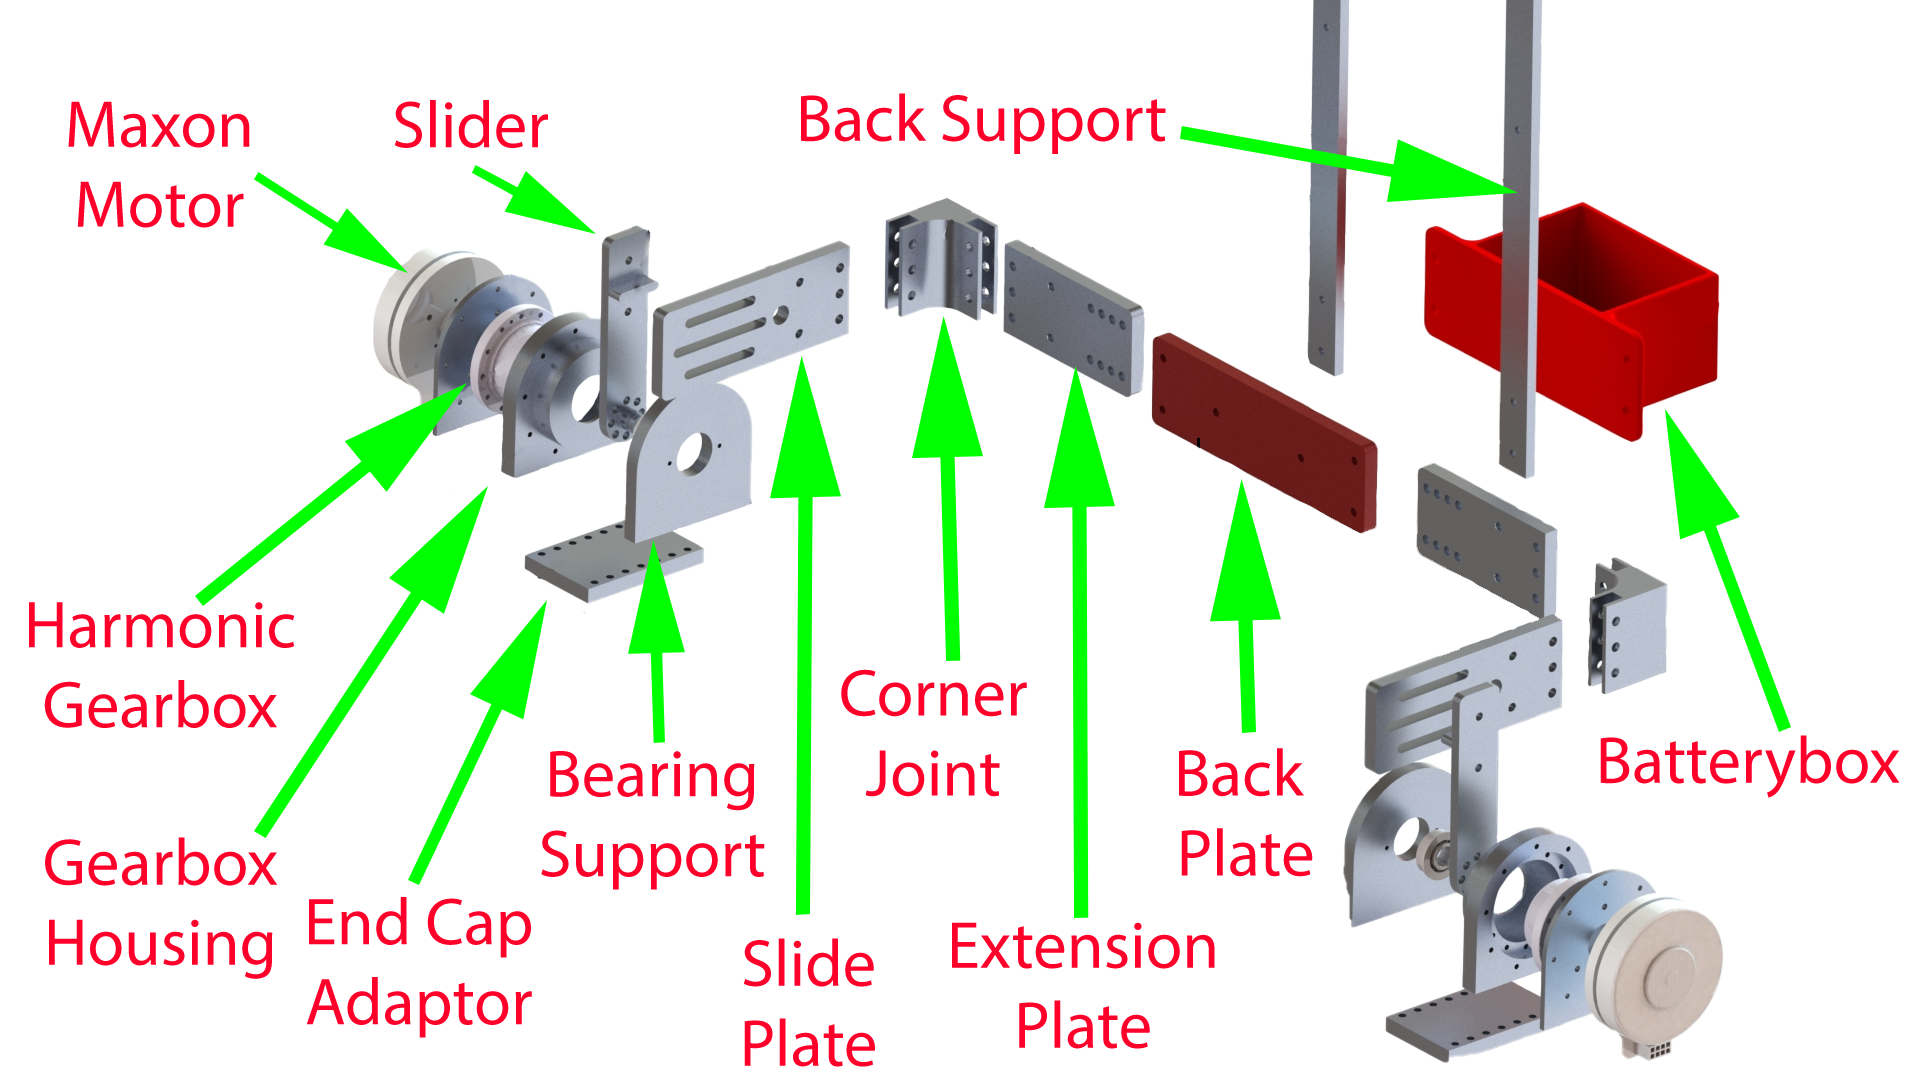
\includegraphics[scale=0.15]{images/mech_design/hip.png}
    \caption{Exploded Hip Mechanism}
    \label{fig:hip}
\end{figure}

LARRE is designed to be either passive or active. The passive mode allows the LARRE to be worn and collect data without controlling the motors. The passive version of the exoskeleton has been built for proof of concept. 

The active mode of the LARRE uses Maxon EC90 flat motors \footnote{https://www.maxongroup.com/maxon/view/product/motor/ecmotor/ecflat/ecflat90/505592} connected to Harmonic gearboxes \footnote{https://www.harmonicdrive.net/products/rotary-actuators#5071}. The Maxon motors are compact and have a low profile and built-in encoders. This motor is ideal for use in exoskeletons since it is a hollowed shaft gearbox that does not increase the exoskeletons' width. The encoders allow for positional control of the motors. Harmonic gearboxes reduce backlash and provide a 100:1 gear ratio. The active mode has been designed but left for future work to implement. 

This platform's modality makes it ideal for testing different orthoses because of its' ability to easily switch the joints to test either a passive or active exoskeleton. The hip also acts as the base for the other joint that will be discussed below. 

